% ============================================================================
% Section 9.5 — Sample Spaces for Compound Events
% CCSS 7.SP.C.8a
% ============================================================================
\section{Sample Spaces for Compound Events}

\begin{stepGoal}
\begin{itemize}
    \item Represent sample spaces using organized lists, tables, and tree diagrams
    \item Count all possible outcomes for compound events
\end{itemize}
\end{stepGoal}

\begin{stepVocabBox}
    \vocabItem{Compound Event}{An event that combines \textbf{two or more} simple events.}
    \vocabItem{Sample Space}{The set of \textbf{all possible outcomes} of an experiment.}
    \vocabItem{Tree Diagram}{A branching picture that shows every possible outcome path.}
\end{stepVocabBox}

\begin{stepsCard}[How to Find a Sample Space for a Compound Event]
    \stepItem{Identify each \textbf{individual event} and its possible outcomes.}
    \stepItem{Choose a method: \textbf{organized list}, \textbf{table}, or \textbf{tree diagram}.}
    \stepItem{List or draw \textbf{every combination} of outcomes --- one from each event.}
    \stepItem{Count the total: total outcomes $=$ (outcomes of event 1) $\times$ (outcomes of event 2).}
\end{stepsCard}

% --- Worked Example 1 ---
\begin{stepExample}{You flip a coin and roll a die. List the sample space.}
    \stepShow{1} Coin: $\{H, T\}$ (2 outcomes). \quad Die: $\{1, 2, 3, 4, 5, 6\}$ (6 outcomes).

    \stepShow{2} Use an organized list.

    \stepShow{3}
    \begin{tabular}{c|cccccc}
     & $1$ & $2$ & $3$ & $4$ & $5$ & $6$ \\ \hline
    $H$ & $H1$ & $H2$ & $H3$ & $H4$ & $H5$ & $H6$ \\
    $T$ & $T1$ & $T2$ & $T3$ & $T4$ & $T5$ & $T6$ \\
    \end{tabular}

    \stepShow{4} Total: $2 \times 6 = 12$ outcomes.
    \stepResult{$12$ outcomes: $H1, H2, \ldots, H6, T1, T2, \ldots, T6$}
\end{stepExample}

% --- Worked Example 2 ---
\begin{stepExample}{A restaurant offers $3$ main dishes (burger, pizza, salad) and $2$ drinks (water, juice). How many different meals can you order?}
    \stepShow{1} Main: $\{B, P, S\}$ (3 outcomes). \quad Drink: $\{W, J\}$ (2 outcomes).

    \stepShow{2} Use a tree diagram (shown as a list).

    \stepShow{3}
    \begin{center}
    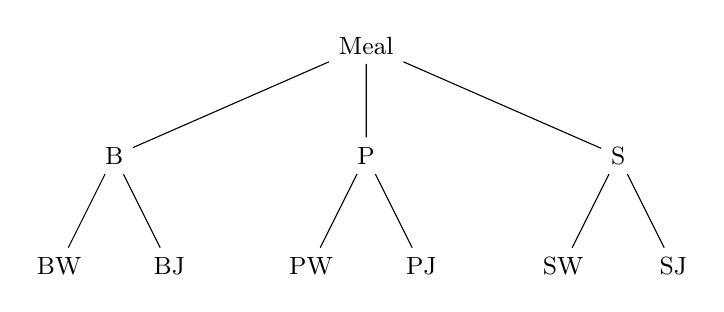
\begin{tikzpicture}[
        level 1/.style={sibling distance=32mm, level distance=14mm},
        level 2/.style={sibling distance=14mm, level distance=14mm},
        every node/.style={font=\small},
        edge from parent/.style={draw, -}
    ]
    \node {Meal}
        child {node {B}
            child {node {BW}}
            child {node {BJ}}
        }
        child {node {P}
            child {node {PW}}
            child {node {PJ}}
        }
        child {node {S}
            child {node {SW}}
            child {node {SJ}}
        };
    \end{tikzpicture}
    \end{center}

    \stepShow{4} Total: $3 \times 2 = 6$ meals.
    \stepResult{$6$ possible meals}
\end{stepExample}

\watchOut{Don't forget any branch! Double-check by multiplying the number of choices for each event.}

% ============================================================================
% PRACTICE
% ============================================================================
\newpage
\begin{stepPractice}{Sample Spaces Practice}
    \resetProblems

    \stepPracticeHeader[step1Color]{Identify the Events}
    \prob You roll two dice. How many outcomes does each die have? \answerBlank[2cm]
    \answer{$6$ each}

    \stepPracticeHeader[step2Color]{Count Total Outcomes}
    \begin{multicols}{2}
    \prob Flip a coin $3$ times. Total outcomes? \answerBlank[2cm]
    \answer{$2 \times 2 \times 2 = 8$}
    \prob Choose $1$ of $4$ shirts and $1$ of $3$ pants. Total outfits? \answerBlank[2cm]
    \answer{$4 \times 3 = 12$}
    \end{multicols}

    \stepPracticeHeader[step3Color]{List the Sample Space}
    \prob You spin a spinner ($A$, $B$) and flip a coin ($H$, $T$). List all outcomes. \answerBlank[4cm]
    \answer{$AH, AT, BH, BT$ (4 outcomes)}

    \wordProblem{A pizza shop offers $2$ crust types (thin, thick) and $3$ toppings (pepperoni, mushroom, olive). Draw a tree diagram or list to find all possible one-topping pizzas. How many are there?}{~}
    \answer{$2 \times 3 = 6$ pizzas: Thin-P, Thin-M, Thin-O, Thick-P, Thick-M, Thick-O}
\end{stepPractice}
